The reliable operation of the different ATLAS systems directly impacts the 
efficiency of the ATLAS experiment 
in recording the $p-p$ collisions delivered by the LHC. 
As a result, high data-taking efficiency is crucial 
for the ATLAS physics program. 

All the ATLAS sub-detectors have operated with a very high efficiency 
($93-95\%$) as shown in Table~\ref{tab:atlas.detstatus} for the 2016 
data taking run.


\begin{table}[!htb]
  \caption{Luminosity weighted relative fraction of good quality data delivery efficiencies (\%) by the various components of the ATLAS 
detector and trigger subsystems during LHC stable beams in $pp$ collisions at $\sqrt{s}=13$ \TeV~with 25 ns bunch spacing between 
April-October 2016, corresponding to a recorded integrated luminosity of 35.9 \ifb. The toroid magnet was off for some runs, 
leading to a loss of 0.7 \ifb.}
\label{tab:atlas.detstatus}
\centering\def\arraystretch{1.2}
\resizebox{\textwidth}{!}{
\begin{tabular}{|c|c|c|c|c|c|c|c|c|c|c|c|}\hline
   \multicolumn{3}{|c|}{Inner Tracker} & 
   \multicolumn{2}{|c|}{Calorimeters} &
   \multicolumn{4}{|c|}{Muon Spectrometer} &
   \multicolumn{2}{|c|}{Magnets} &
   Trigger\\\hline
Pixels & SCT & TRT & LAr & Tile & MDT & RPC & CSC & TGC & Solenoid & Toroid & L1\\ \hline
98.9 & 99.9 & 99.7 & 99.3 & 98.9 & 99.8 & 99.8 & 99.9 & 99.9& 99.1 & 97.2 & 98.3 \\ \hline \hline
\multicolumn{12}{|c|}{Good for physics: 93-95\% (33.3-33.9 \ifb)} \\
\hline\hline\end{tabular}}
\end{table}

% https://twiki.cern.ch/twiki/bin/view/AtlasPublic/RunStatsPublicResults2010


The ATLAS recorded efficiency in 2016 is over 90\%, as shown in 
Figure \ref{fig:tdaq_diagram} with a negligible fraction of data loss due to 
the ATLAS DAQ system. 
The ATLAS dataflow architecture is scaling well with the increased 
instantaneous luminosity during 2016 data-taking and is capable of handling 
larger pileup ($<\mu>$) and thus larger event sizes.
For illustration,  Figure \ref{fig:run_pileup} shows the evolution of the 
average processing time per event and 
the event size where there is relatively mild increase as a function of pileup 
which is well within the system capacity.

\begin{figure}[t!]
%\vspace{-0.5cm}
\centering
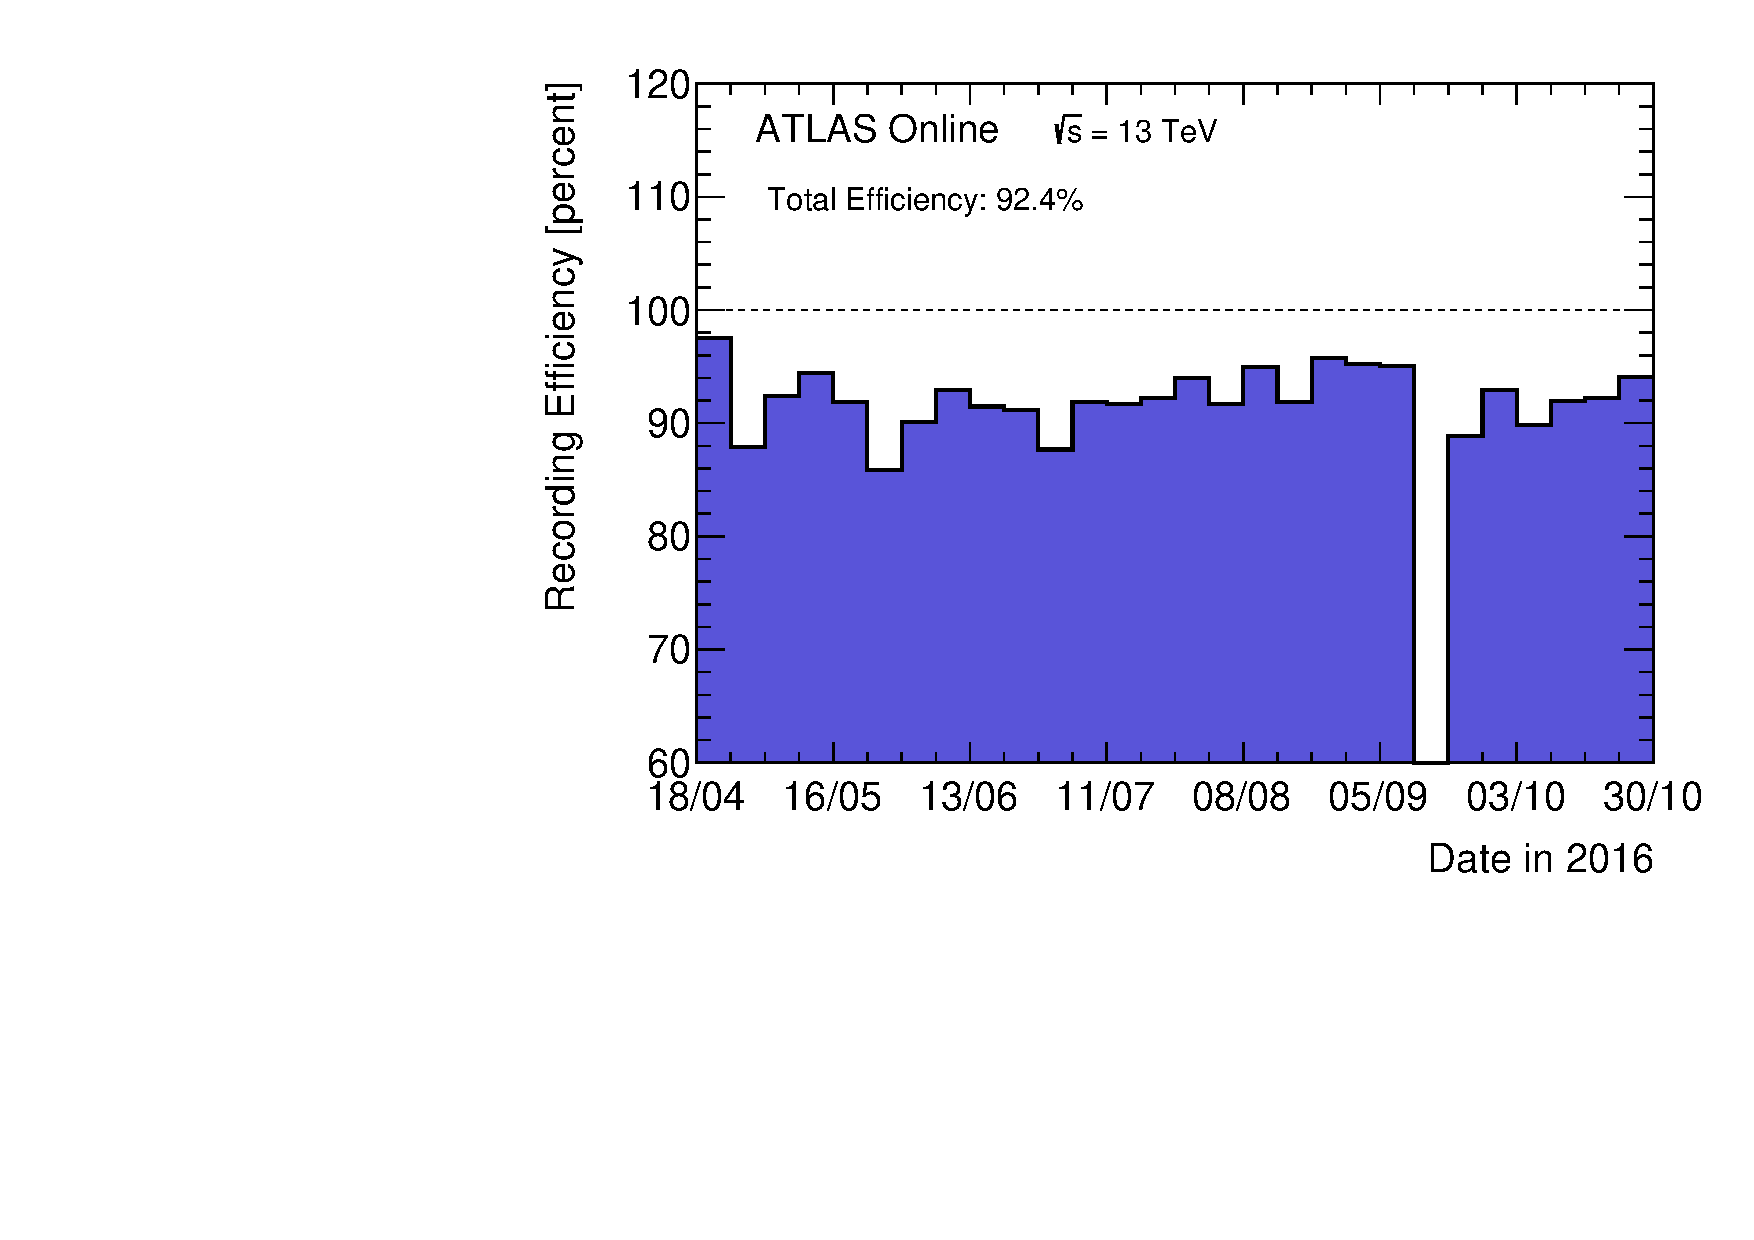
\includegraphics[width=0.75\textwidth]{recEffByWeek} 
\caption{ATLAS recorded efficiency \cite{atlasTwiki}.}
\label{fig:tdaq_diagram}
\end{figure} 


\begin{figure}[t!]
%\vspace{-0.1cm}
\centering
\begin{subfigure}[t]{0.48\textwidth}
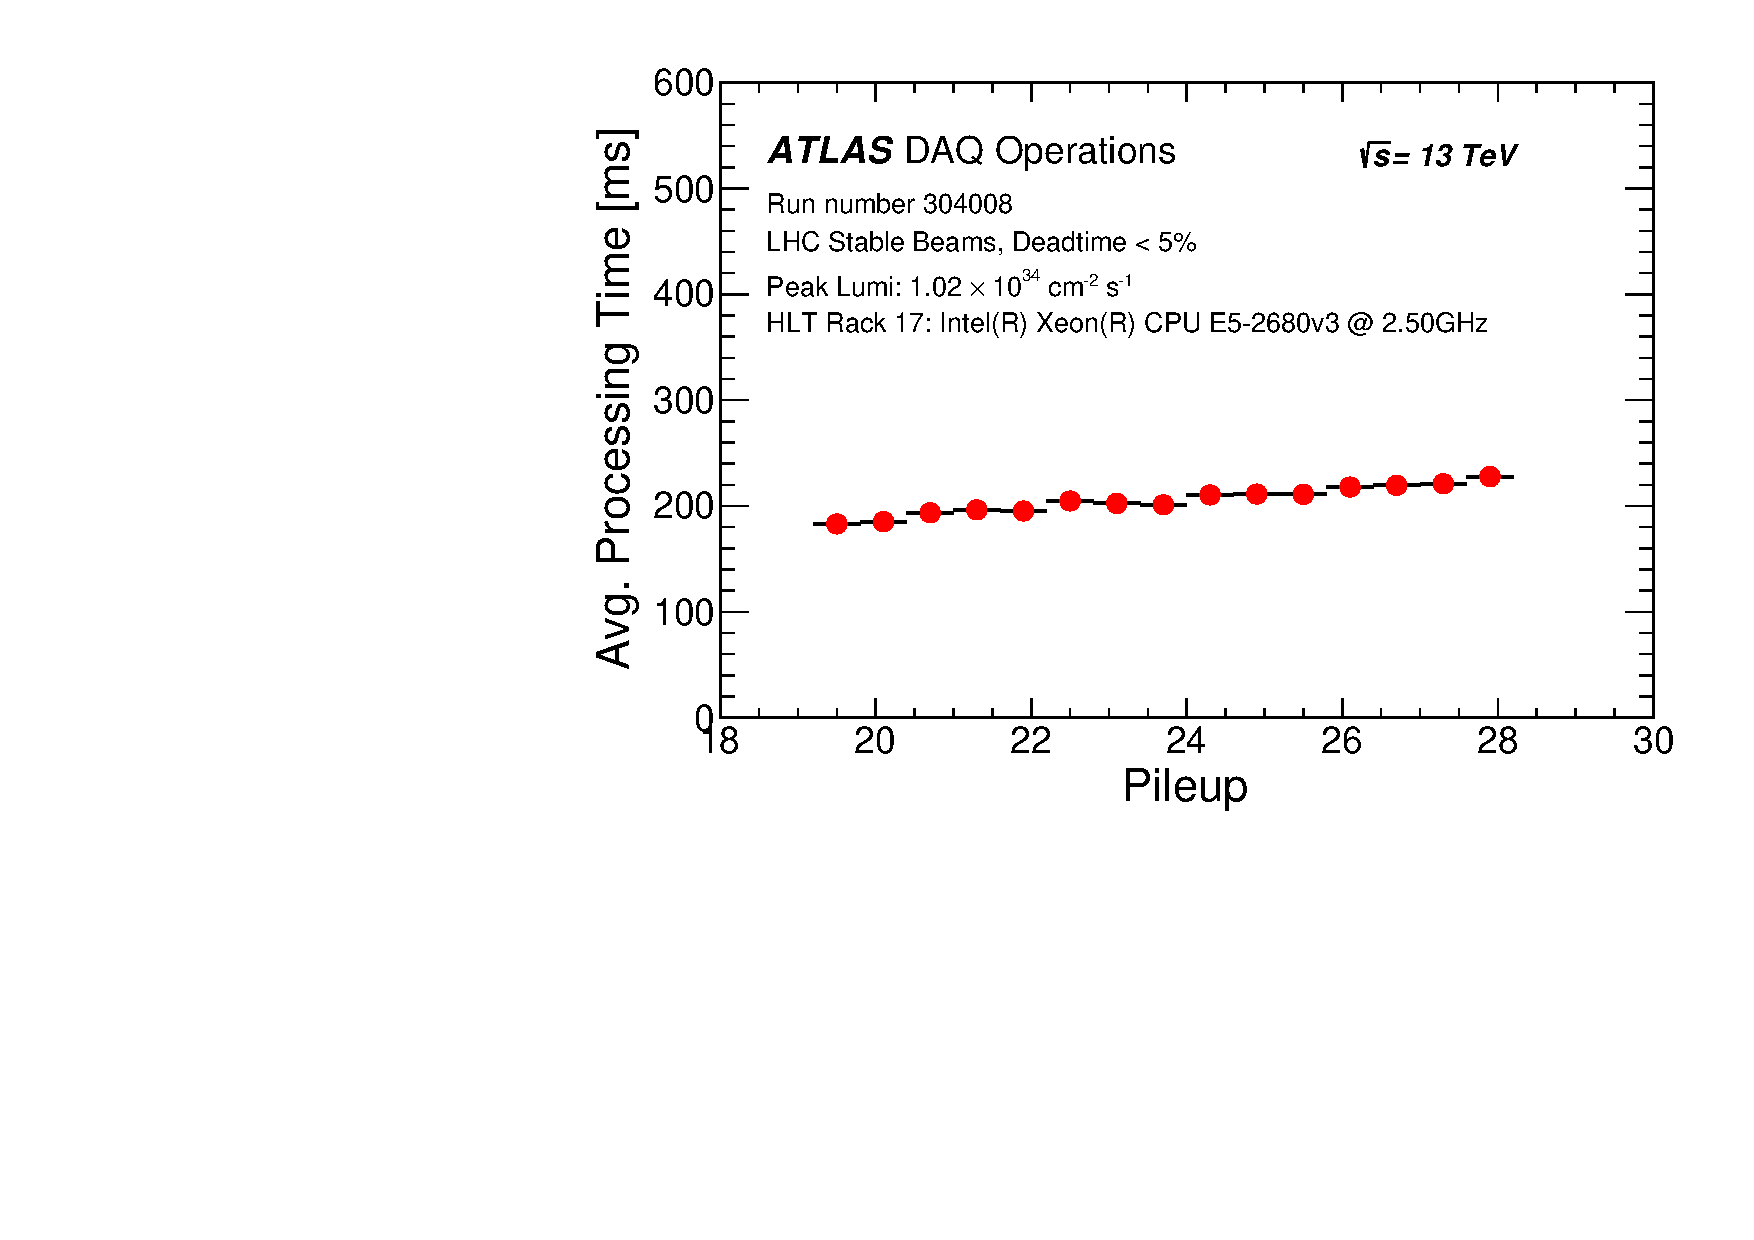
\includegraphics[width=.95\textwidth]{hProf_run_304008_pileup_AvgProcessingTime.pdf}
\end{subfigure}
\begin{subfigure}[t]{0.48\textwidth}
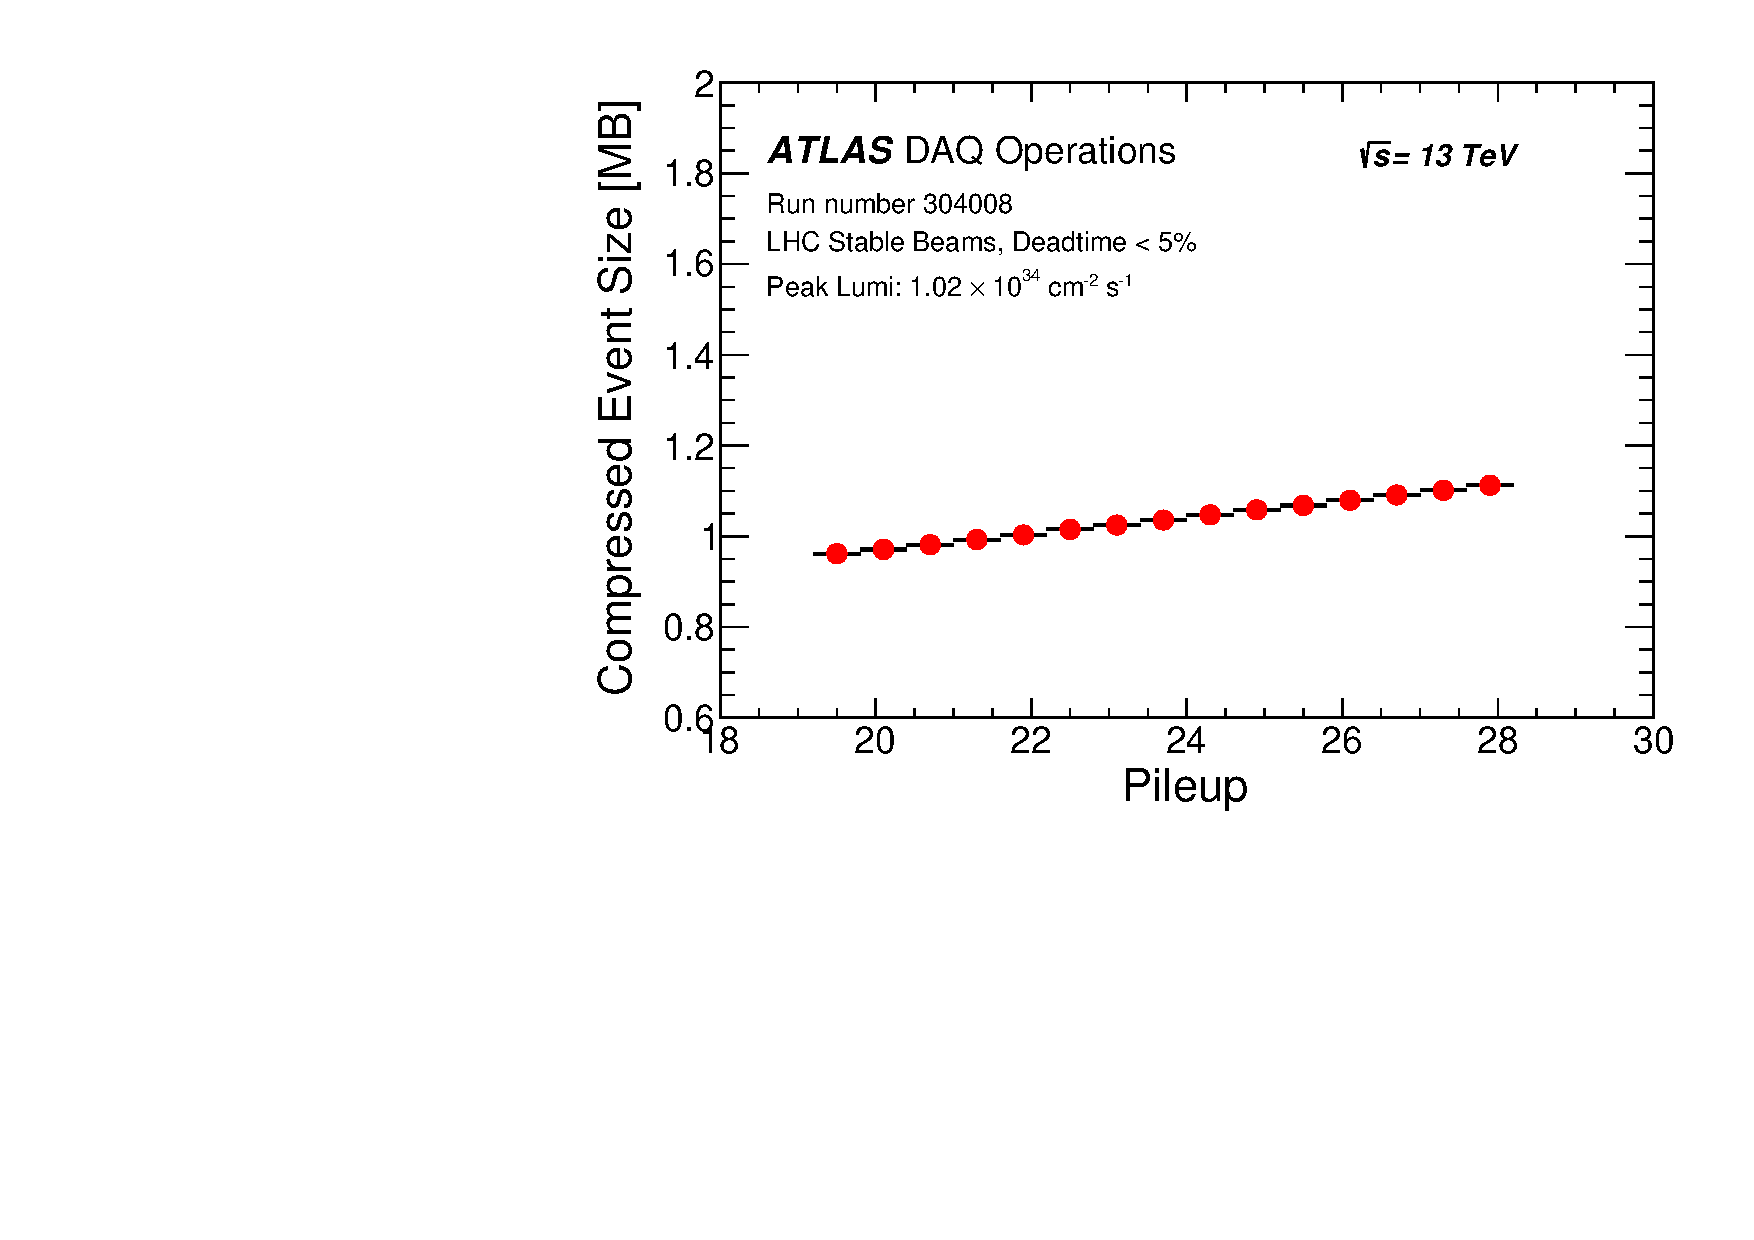
\includegraphics[width=.95\textwidth]{hProf_run_304008_pileup_EventSize.pdf}
\end{subfigure}
\vspace{-0.3cm}
\caption{Performance in Run 2: Average processing time as a function of pileup (left), compressed event size as a function of pileup (right).}
\label{fig:run_pileup}
\end{figure} 



As a result of this excellent performance of all the sub-detectors,
ATLAS has recorded  almost 92\% of the luminosity delivered by the LHC during 
2015 and 2016 as illustrated in  Figure~\ref{fig:exp.op.intlumi}.
The total integrated luminosity used in this analysis after 
applying a large number of checks amounts to 
 36.1 \ifb~ divided between 3.2 \ifb~in 2015 and 32.9 \ifb~in 2016.

\begin{figure}[t!]
%\vspace{-0.1cm}
\centering
\begin{subfigure}[t]{0.48\textwidth}
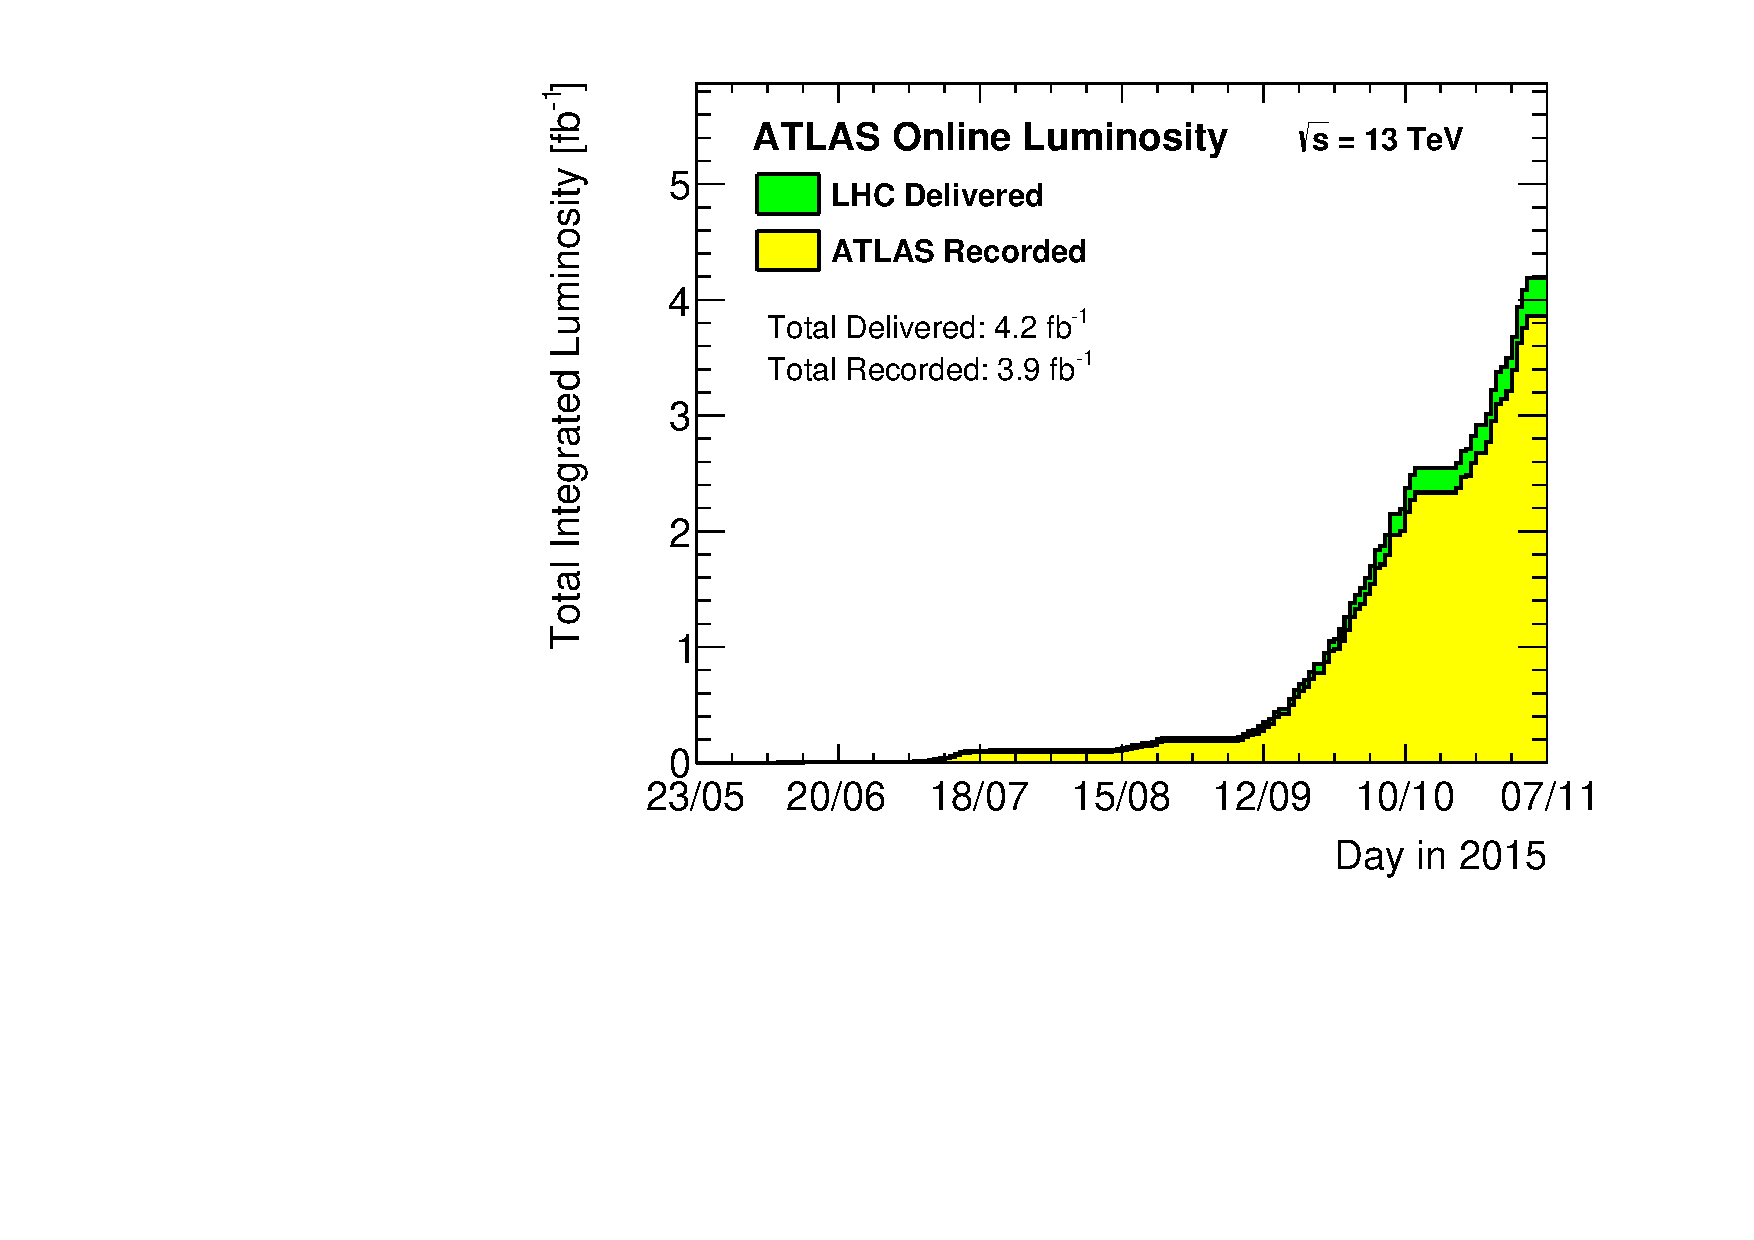
\includegraphics[width=.95\textwidth]{sumLumiByDay2015}
\subcaption{2015}
\end{subfigure}
\begin{subfigure}[t]{0.48\textwidth}
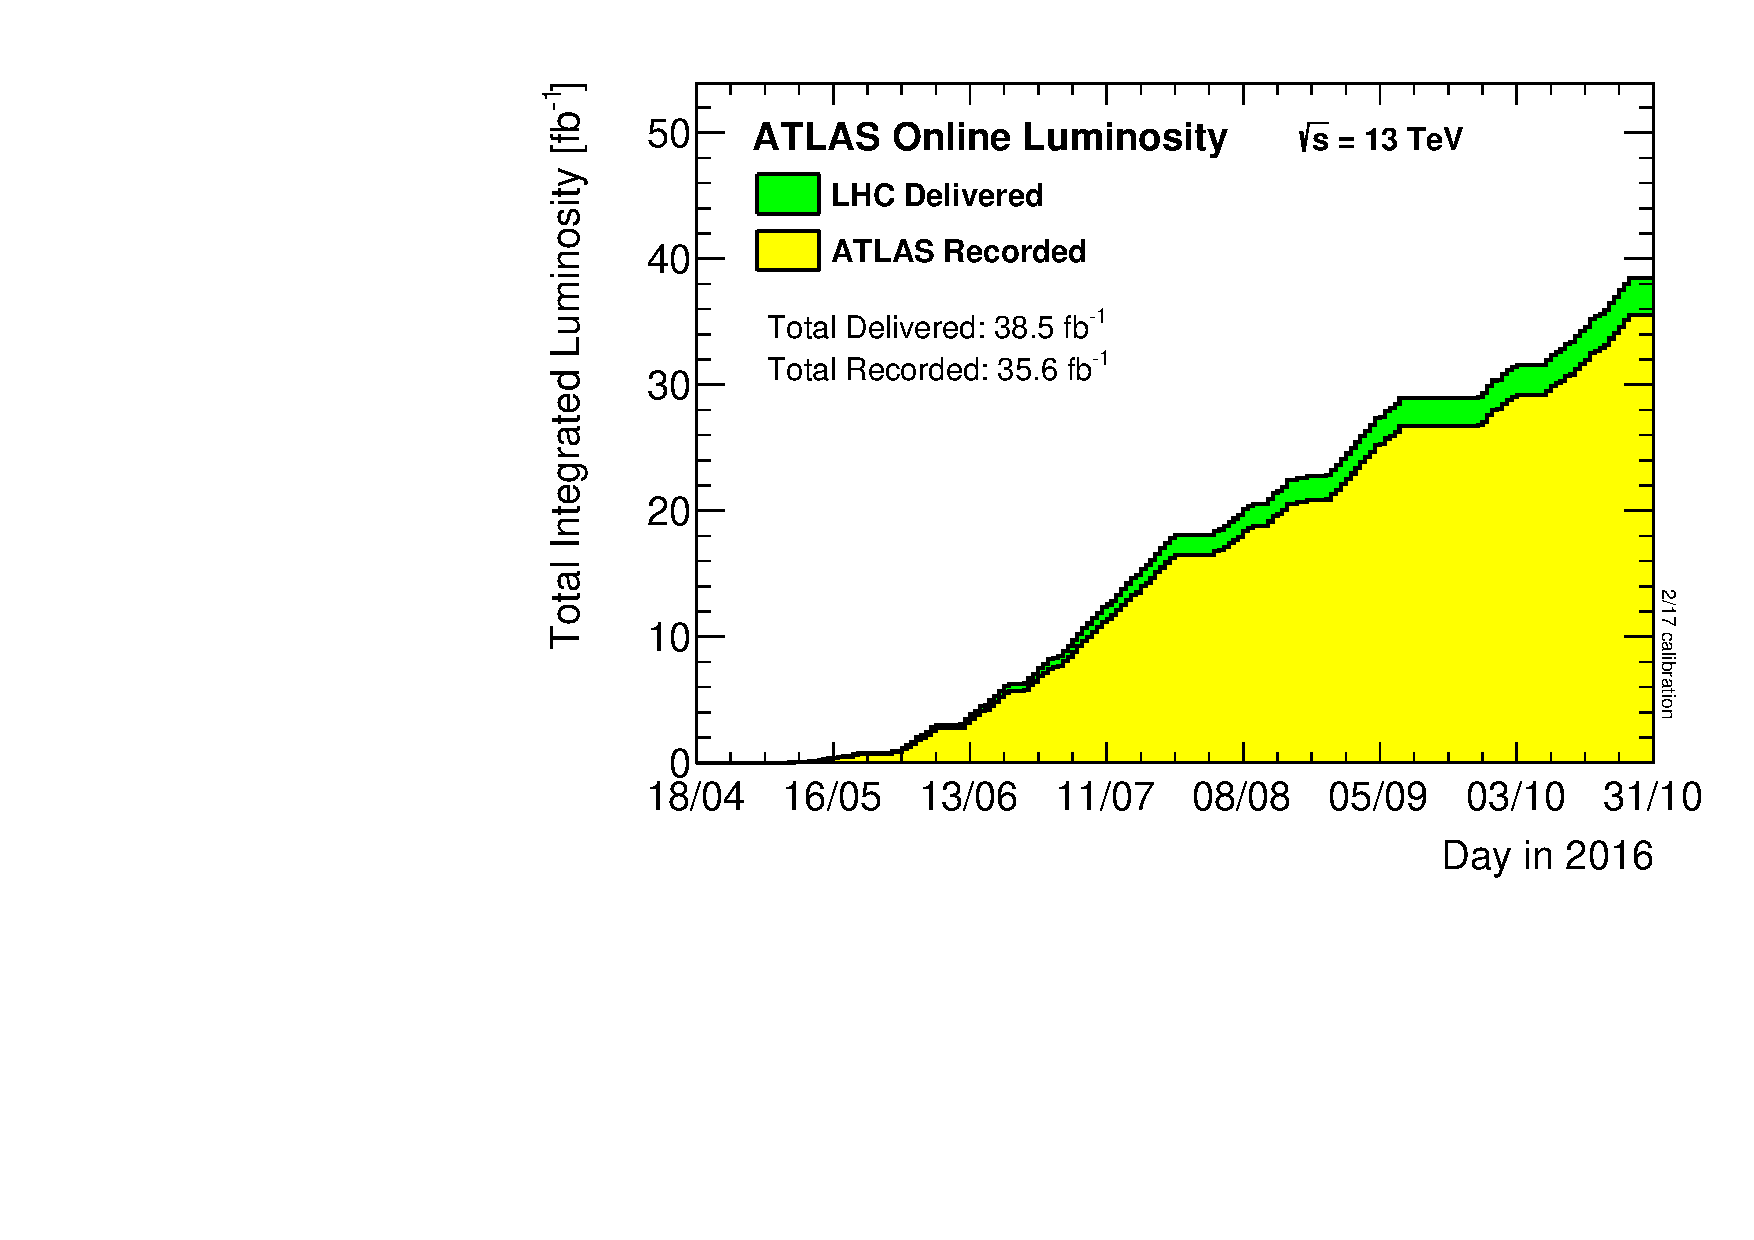
\includegraphics[width=.95\textwidth]{sumLumiByDay2016}
\subcaption{2016}
\end{subfigure}
\vspace{-0.3cm}
\caption{
Cumulative luminosity versus time delivered to (green) and recorded by ATLAS 
(yellow) during stable beams for pp collisions at 13 \TeV~centre-of-mass energy 
in (a) 2015 and (b) 2016.
}
\label{fig:exp.op.intlumi}
\end{figure} 


